\documentclass[11pt,a4paper]{scrartcl}
\typearea{12}
\usepackage{graphicx}
\usepackage{pstricks}
\usepackage{listings}

\pagestyle{headings}
\markright{Computational Neuroscience - information theoty}
\begin{document}

\subsection*{Introduction}
These notes are about information theory and spike trains; they were
part of the course last year, this year they are included only for
interest.

\subsection*{Information and its application to spike train data.}

Information theory is a large and impressive subject so this one
lecture is intended only as the broadest overview. The subject is
lucky to have an excellent textbook - Cover and Thomas - and you
should look there for more details.

The key insight in information theory is to think about randomness in
the right way. Imagine you are applying for a job and you have to fill
in your final grade; for simplicity a first, a second or a third, on
the application form. Now, your grade isn't random, there might be a
random element, but it is also the result of your ability to do well
in exams, of how hard you prepared and possible of whatever
difficulties around the exam time might have prevented you performing
at your best. Furthermore, your potential employer is interested in
your grade precisely because it isn't random, it is something they
believe is an indication of how well you will do the job. However,
until they read what you have written they do not know your grade and
so, to them, it is like performing a random experiment and it can be
modelled using a random variable.

In fact, most situation we use a random variable for are like this;
the variable models something we don't know rather than something that
is truly random. The example of a coin flip often used when
describing random variables is misleading. 

Now, returning to the scenario above, consider how much the potential
employer learns from reading your grade. This, of course, depends on
how well the grading is aligned to the potential employer's, that is a
complicated question, but there is a simpler issue related to the
randomness of the variable, the degree to which the potential employer
can't guess the answer before reading what is written. 

Think about how exams are marked. In America they are marked \lq{}to a
curve\rq{}; we don't do that here and the description here isn't a
picture of how exams are marked, it is just used to motivate
information theory. In a cartoon sketch of marking to a curve,
everyone is marked and the grades fall into a normal curve and two
divisions are made at the points where the curves are steepest
dividing those who took the exam into three groups, firsts, seconds
and thirds. For definiteness say the distribution of marks is 
\begin{equation}
p(x)=\frac{1}{\sqrt{2\pi\sigma^2}}e^{-(x-\mu)^2/2\sigma^2}
\end{equation}
and the divisions are made at $x=\mu\pm\sigma$ then $68.3\%$ of
students will get a second, $15.9\%$ will get either a first or a
third. This is described in Figure 1.

\begin{figure}
\begin{center}
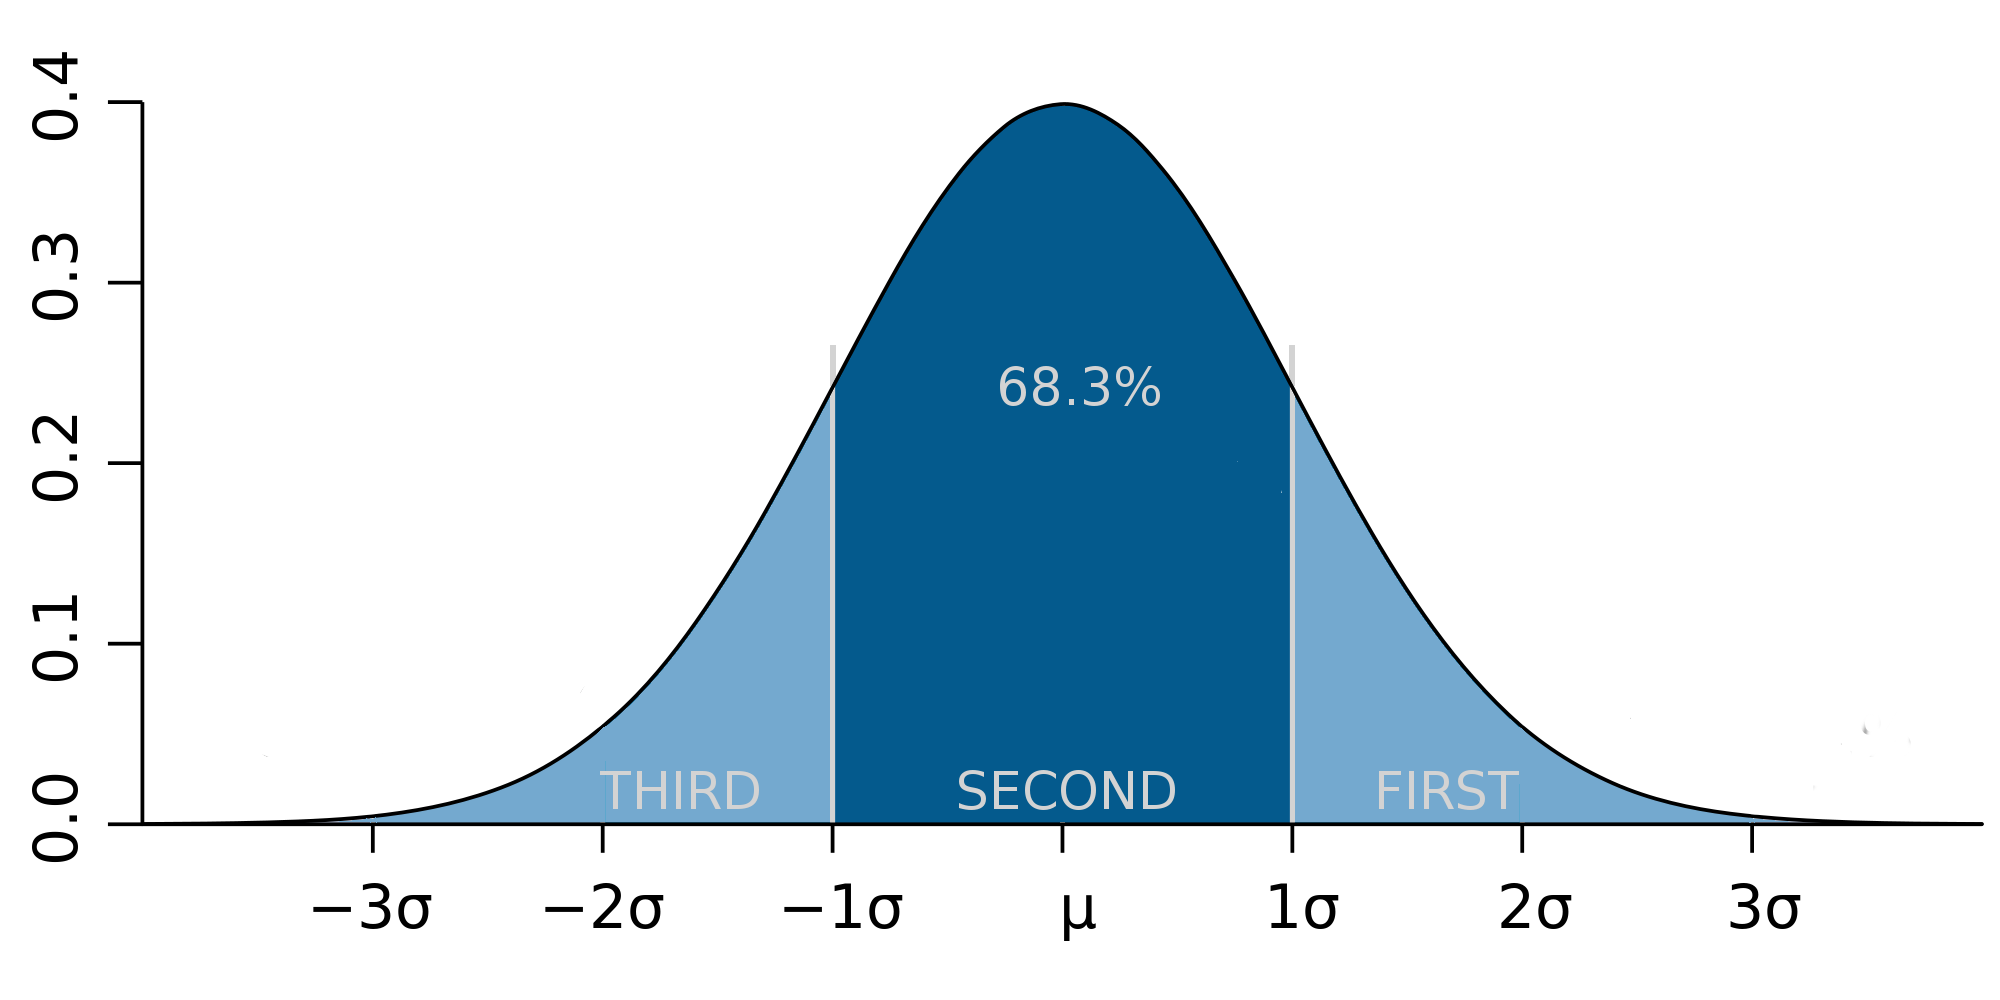
\includegraphics[width=7cm]{marked_to_curve.png}
\end{center}
\caption{A simplified picture of marking to a curve.}
\end{figure}

Now, think of the potential employer: sometimes when they ask what
grade a prospective employee got they will find out something very
significant, if the student got a first they are in the top $15.9\%$
of exam takers, if they got a third they are in the bottom $15.9\%$;
however, most of the time, almost seven times in ten, $68.3\%$ of the
time to be exact, they will learn that the student got a second. This
isn't very informative, it just says the student got the same grade as
$68.3\%$ of students. Thus, although some of the time the prospective
employer learns something very informative, most of the time they
learn that the student is about the same as most students. On average
this isn't a very informative distribution. 

\textsl{Shannon's Entropy} was introduced by Claude Shannon in his 1948 papers,
two papers which basically created the field of information theory. It
is a single quantity that measures this idea of informativeness,
balancing how useful a piece of information is with how likely you are
to get it. For a finite discrete distribution with random variable $X$,
possible outcomes $\{x_1,x_2,\ldots x_n\}\in\mathcal{X}$ and
probabilities $p_X(x_i)$, the entropy is
\begin{equation}
H(X)=-\sum_{x_i\in \mathcal{X}}{p(x_i)\log_2p(x_i)}
\end{equation}

This might seem like a strange definition of information, but it turns
out there is an important theorem supporting it. This links the
entropy to the compressibility of the outcomes; setting up this
theorem would take too long so here is a quick version. 

Imagine storing a long sequence made up of the letters A, B, C and D
as binary. The obvious way to do it would be to say that there are
four letters so the sequence should be stored using two bits, a
dictionary might look like
\begin{center}
\begin{tabular}{cccc}
A&B&C&D\\
\hline
00&01&10&11
\end{tabular}
\end{center}
so the sequence AABC would be stored as 00000110, splitting this up
into two: 00 00 01 10 allows the binary to be converted back into the
original letters. Moreover, since each letter is coded using two bits,
it is clear the code length is twice the number of letters. 

Now, say we also knew that $p($A$)=0.5$, $p($B$)=0.25$,
$p($C$)=p($D$)=0.125$, in other words, in the message that will be
encoded, A occurs half the time, B a quarter the time and C and D an
eighth of the time. Now, consider this dictionary
\begin{center}
\begin{tabular}{cccc}
A&B&C&D\\
\hline
0&10&110&111
\end{tabular}
\end{center}
Here, the sequence AABC become 010110110, this can be split up into 0
10 110 110 because the code word 0 is the only code word beginning
with 0 and the code word 10 is the only one beginning with 10. Now,
some of the code words are longer than two, but, since A occurs half
the time and has a code word of length one, B occurs a quarter the
time and has a code word of length two and C and D each occur an
eighth the time with code words of length three, the average code
length for each letter is $0.5\times 1 +0.25\times 2 + 0.125\times 3 +
0.125\times 3=1.75$. This is the same as the entropy
\begin{equation}
H(X)=-0.5\log_2(0.5)-0.25\log_2(0.25)-0.125\log_2(0.125)-0.125\log_2(0.125)=1.75
\end{equation}
It doesn't always work out exactly the same, but the theorem says that
the entropy is a basic limit on compressibility and that the best code
attains or nearly attains this limit. Basically it works because
\begin{equation}
H(X)=-\sum_{x_i\in \mathcal{X}}{p(x_i)\log_2p(x_i)}
\end{equation}
can be thought of as calculating the average value of $-\log_2p(x_i)$
and an even that is twice as rare contains one more bit of
information.

It is worth making two other quite remarks about the suitability of
the Shannon entropy. The first is that it can always be calculated; it
isn't always possible to find an average. Imagine you have measured
heights, up to a one centimetre tolerance, so you have a discrete
distribution for how high people are in a whole number of centimetres. It is possible to find the average height
\begin{equation}
<X>=\sum_{x_i\in\mathcal{X}}x_ip_X(x_i)
\end{equation}
because we are able to multiply heights by a scalar, in this case the
corresponding probability and we can add the results. However, if we
were looking at fruit purchased in a supermarket, the average fruit
would make no sense since we would not know how to work out
\begin{equation}
0.25\times \mbox{apple}+0.125\times \mbox{banana}+0.1\times \mbox{pear}\ldots
\end{equation}
However, no matter what the elements of $\mathcal{X}$ are, if we are
dealing with a probability space, each element has a probability and a
probability is a thing that can be added and so on. One slight subtlety is that some $x_i$ might have the value zero and 
\begin{equation}
\lim_{\rho \rightarrow 0}\log{\rho}=-\infty
\end{equation}
However, 
\begin{equation}
\lim_{\rho \rightarrow 0}\rho\log{\rho}=0
\end{equation}
and what is in the entropy is $p(x_i)\log_2{p(x_i)}$ so we just take
this to be zero when $p(x_i)=0$. The second point is that the
appearance of the logarithm is providential; probabilities often
involve products, if $X$ and $Y$ are independent probability
distributions then the probability that $X=x$ and $Y=y$ is
$p_X(x)p_Y(y)$, for example. Products can be difficult to deal with in
theorems, but logarithms turn products in to sum:
\begin{equation}
\log_2{ab}=\log_2{a}+\log_2{b}
\end{equation}

Anyway, back to exam grade example. The distribution we looked at has
\begin{equation}
H(X)=-0.684\log_2{.684}-0.386\log_2{0.159}=1.4
\end{equation}
If, instead, the division between the grades were arranged so that an equal number of people got a first, second and third then the probability would be 
\begin{equation}
p(\mbox{first})=p(\mbox{second})=p(\mbox{third})=\frac{1}{3}
\end{equation}
and
\begin{equation}
H(X)=-\log_2\frac{1}{3}=1.58
\end{equation}
In fact, the constant distribution where all outcomes are equally
likely is always the most informative, if there are $n$ outcomes and all have the same probability: $p(x_i)=1/n$ then
\begin{equation}
H(X)=\sum_{i=1}^np(x_i)\log_2{p(x_i)}=\log_2{n}
\end{equation}
This makes sense, if all outcomes are equally likely then the outcome
is completely unpredictable and learning the outcome is maximally
informative. Conversely, if only one outcome ever occurs then
$p(x_i)=1$ for one value of $i$ and $p(x_i)=0$ for all the others, in
this case $H(X)=0$ since $\log_21=0$ and we have already decided
$0\log_20=1$. This makes sense, if you already know the outcome, you
don't learn anything from learning what the outcome was. If there are
two outcomes, $a$ and $b$ with $p(a)=p$ and $p(b)=1-p$ then the entropy is
\begin{equation}
H=-p\log_2{p}-(1-p)\log_2{(1-p)}
\end{equation}
which is plotted as Figure 2.

\begin{figure}
\begin{center}
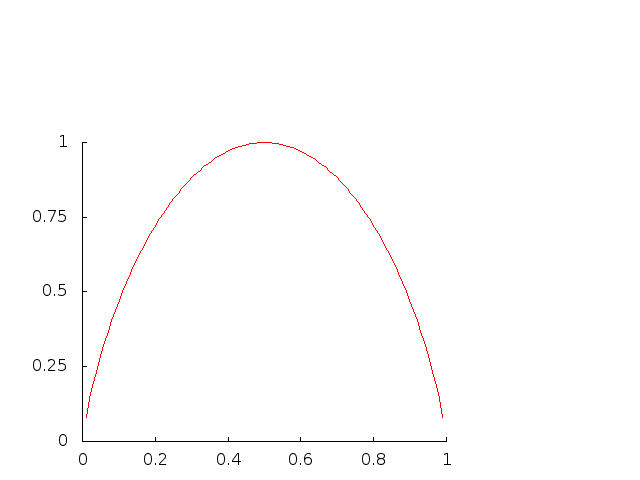
\includegraphics[width=7cm]{info_one_d.png}
\end{center}
\caption{Information with two outcomes.}
\end{figure}


Now, what about electrophysiological data? The problem with applying
electrophysiological data to spike trains is that the theory we have
looked at applies to discrete distributions whereas spike trains live
in a continuous space. In fact there is a version of information
theory for continuous variables, it is trickier to use, but that isn't
the real problem, the problem is that spike trains aren't easily
described by the sort of variables that would be useful for working
out the information. The answer, first developed by Bialek and co-workers is
to discretize the spike trains. 

It is easier to describe what Bialek and co-workers did if we first
briefly describe the data they applied it to; however, the ideas are,
in principle, applicable to a wide range of situations even if, in
practise, the fly system they use is very suitable from the point of
view of producing a sufficient amount of data. Flies have a very rapid
response to moving visual stimuli, this is important, for example, as
part of their escape response to predation. Spikes are recorded from
one of the large vision neurons in blowfly while they are being to
exposed to random moving visual stimuli with a statistical structure
which mimic the natural visual environment of flies.

Since the reaction time of a blowfly to visual data of this sort is
about 30 ms the total stimulus is split up into 30 ms windows. These
fragments of spike trains are regarded as the outcomes whose
information will be calculation. These 30 ms fragments are then mapped
to binary words by bining the spikes trains over small time bins, so,
for example, if the bin size was 2 ms then it might look like Figure
3. Of course, for the binary words to actually be binary there can be
at most one spike in each bin, this should happen provided the bin
size is less than the refractory period.

\begin{figure}
\begin{center}
\setlength{\unitlength}{3000sp}%
%
\begingroup\makeatletter\ifx\SetFigFont\undefined%
\gdef\SetFigFont#1#2#3#4#5{%
  \reset@font\fontsize{#1}{#2pt}%
  \fontfamily{#3}\fontseries{#4}\fontshape{#5}%
  \selectfont}%
\fi\endgroup%
\begin{picture}(6793,2767)(1789,-5945)
\thinlines
{\color[rgb]{0,0,0}\put(1801,-4111){\line( 1, 0){6750}}
}%
\thicklines
{\color[rgb]{0,0,0}\put(4276,-3211){\line( 0,-1){900}}
}%
{\color[rgb]{0,0,0}\put(7381,-3211){\line( 0,-1){900}}
}%
{\color[rgb]{0,0,0}\put(2521,-3211){\line( 0,-1){900}}
}%
\thinlines
{\color[rgb]{0,0,0}\put(2251,-5821){\line( 0,-1){ 90}}
}%
{\color[rgb]{0,0,0}\put(2701,-5821){\line( 0,-1){ 90}}
}%
{\color[rgb]{0,0,0}\put(3151,-5821){\line( 0,-1){ 90}}
}%
{\color[rgb]{0,0,0}\put(4051,-5821){\line( 0,-1){ 90}}
}%
{\color[rgb]{0,0,0}\put(4501,-5821){\line( 0,-1){ 90}}
}%
{\color[rgb]{0,0,0}\put(4951,-5821){\line( 0,-1){ 90}}
}%
{\color[rgb]{0,0,0}\put(5401,-5821){\line( 0,-1){ 90}}
}%
{\color[rgb]{0,0,0}\put(5851,-5821){\line( 0,-1){ 90}}
}%
{\color[rgb]{0,0,0}\put(6301,-5821){\line( 0,-1){ 90}}
}%
{\color[rgb]{0,0,0}\put(6751,-5821){\line( 0,-1){ 90}}
}%
{\color[rgb]{0,0,0}\put(7201,-5821){\line( 0,-1){ 90}}
}%
{\color[rgb]{0,0,0}\put(7651,-5821){\line( 0,-1){ 90}}
}%
{\color[rgb]{0,0,0}\put(8101,-5821){\line( 0,-1){ 90}}
}%
{\color[rgb]{0,0,0}\put(8551,-5821){\line( 0,-1){ 90}}
}%
\thicklines
{\color[rgb]{0,0,0}\put(5176,-4336){\vector( 0,-1){900}}
}%
\thinlines
{\color[rgb]{0,0,0}\put(1803,-5843){\line( 0,-1){ 90}}
}%
{\color[rgb]{0,0,0}\put(1820,-5916){\line( 1, 0){6750}}
}%
{\color[rgb]{0,0,0}\put(3603,-5814){\line( 0,-1){ 90}}
}%
\put(1908,-5871){\makebox(0,0)[lb]{\smash{{\SetFigFont{29}{34.8}{\rmdefault}{\mddefault}{\updefault}{\color[rgb]{0,0,0}0}%
}}}}
\put(2358,-5871){\makebox(0,0)[lb]{\smash{{\SetFigFont{29}{34.8}{\rmdefault}{\mddefault}{\updefault}{\color[rgb]{0,0,0}1}%
}}}}
\put(2808,-5871){\makebox(0,0)[lb]{\smash{{\SetFigFont{29}{34.8}{\rmdefault}{\mddefault}{\updefault}{\color[rgb]{0,0,0}0}%
}}}}
\put(3258,-5871){\makebox(0,0)[lb]{\smash{{\SetFigFont{29}{34.8}{\rmdefault}{\mddefault}{\updefault}{\color[rgb]{0,0,0}0}%
}}}}
\put(3708,-5871){\makebox(0,0)[lb]{\smash{{\SetFigFont{29}{34.8}{\rmdefault}{\mddefault}{\updefault}{\color[rgb]{0,0,0}0}%
}}}}
\put(4158,-5871){\makebox(0,0)[lb]{\smash{{\SetFigFont{29}{34.8}{\rmdefault}{\mddefault}{\updefault}{\color[rgb]{0,0,0}1}%
}}}}
\put(4608,-5871){\makebox(0,0)[lb]{\smash{{\SetFigFont{29}{34.8}{\rmdefault}{\mddefault}{\updefault}{\color[rgb]{0,0,0}0}%
}}}}
\put(5058,-5871){\makebox(0,0)[lb]{\smash{{\SetFigFont{29}{34.8}{\rmdefault}{\mddefault}{\updefault}{\color[rgb]{0,0,0}0}%
}}}}
\put(5508,-5871){\makebox(0,0)[lb]{\smash{{\SetFigFont{29}{34.8}{\rmdefault}{\mddefault}{\updefault}{\color[rgb]{0,0,0}0}%
}}}}
\put(5958,-5871){\makebox(0,0)[lb]{\smash{{\SetFigFont{29}{34.8}{\rmdefault}{\mddefault}{\updefault}{\color[rgb]{0,0,0}0}%
}}}}
\put(6408,-5871){\makebox(0,0)[lb]{\smash{{\SetFigFont{29}{34.8}{\rmdefault}{\mddefault}{\updefault}{\color[rgb]{0,0,0}0}%
}}}}
\put(6858,-5871){\makebox(0,0)[lb]{\smash{{\SetFigFont{29}{34.8}{\rmdefault}{\mddefault}{\updefault}{\color[rgb]{0,0,0}0}%
}}}}
\put(7308,-5871){\makebox(0,0)[lb]{\smash{{\SetFigFont{29}{34.8}{\rmdefault}{\mddefault}{\updefault}{\color[rgb]{0,0,0}1}%
}}}}
\put(7758,-5871){\makebox(0,0)[lb]{\smash{{\SetFigFont{29}{34.8}{\rmdefault}{\mddefault}{\updefault}{\color[rgb]{0,0,0}0}%
}}}}
\put(8208,-5871){\makebox(0,0)[lb]{\smash{{\SetFigFont{29}{34.8}{\rmdefault}{\mddefault}{\updefault}{\color[rgb]{0,0,0}0}%
}}}}
\end{picture}%

\end{center}
\end{figure}

Now, when the whole data set is discretized we can count how often
each 'word', that is each sequence of zeros and ones, occurs allowing
the probability for that word to be estimated:
\begin{equation}
p(w)\approx \frac{\#\mbox{occurrences of }w}{\#\mbox{all words}}
\end{equation}
With these probabilities it is possible to estimate the entropy of the
data
\begin{equation}
H(X)\approx -\sum_{w_i\in\mathcal{W}}p(w_i)\log_2{p(w_i)}
\end{equation}
where $\mathcal{W}$ is the set of all words. Now, obviously, one
difficulty with this is that the $\mathcal{W}$ is huge, if the bin size is 2 ms and the word length 30 ms then 
\begin{equation}
|\mathcal{W}|=2^{15}=32768
\end{equation}
so a huge amount of data is needed to accurately estimate the
probabilities. If we believe a higher resolution is needed to capture
the information present in the spike trains, or if the time scale
stimuli are integrate over is longer, this become ginormous, for 50 ms
at 1 ms resolution, for example,
\begin{equation}
|\mathcal{W}|=2^{50}=1125899906842624
\end{equation}
There are ways to address this, by extrapolating to high resultion
from lower ones, or using a clever Baysian approach based.

Leaving the estimation problem aside, in looking at spike trains we
are interested in the information they carry about the stimulus. The
randomness in the spike trains comes in two forms; the useful
randomness we have been discussing where the randomness of the spike
train is related to the randomness of the stimulus; by actually
recording the spike train we are learning something about the
stimulus. There is also randomness that is uninformative in this
context, the result of the neuron receiving multiple inputs from other
neurons which may be engaged in other processing tasks, and possibly
from the neuron itself being involved in other roles as well as begin
part of the neural pathway encoding and decoding this specific visual
stimulus. This uninteresting randomness is the information still
present in the spike trains when the stimulus is known. If $W$
represents the spike trains and $S$ the stimulus, this is called
$H(W|S)$.

Here $H(W|S)$ is calculated by repeating the same stimulus sequence
many times so for each of the 30 ms fragments there is enough
repititions to estimate $p(w_i|\mbox{given stimulus }s)$ the
probability of $w_i$ for a given stimulus. This gives the entropy
$H(W|\mbox{given stimulus }s)$. This is then averaged over all the
stimuli to give $H(W|S)$. $H(W)$ is also calculated by calculating
$p(w_i)$ in the usual way: note the difference, $H(W|\mbox{given
  stimulus }s)$ is calculated by looking at the distribution of
responses to a specific stimulus, this is then averaged over all
stimuli to get $H(W|S)$ whereas $H(W)$ is calculated by looking at all
responses to all the stimuli. Now, we are interested in the
information about the stimuli contained in the spike train so we look
at $H(W)-H(W|S)$, the information in the spike trains minus the
information, that is the randomness, remaining when the stimulus is
known. 

This quantity is known as the \textsl{mutual information}
\begin{equation}
I(W,S)=H(W)-H(W|S)
\end{equation}
It is a measure of how much information $W$ contains about $S$. It
isn't obvious from the description given here but the mutual information is symmetric
\begin{equation}
H(W)-H(W|S)=I(W,S)=I(S,W)=H(S)-H(S|W)
\end{equation}

The idea behind looking at information in spike trains is that it
might be a tool for understanding coding. For example, in the case of
blowfly, it has been shown that there is information in spike trains
at sub-milisecond scales, which is smaller than the temporal structure
of the stimulus. This implies that spike timing plays a role in coding
in a way that goes beyond just indicating the timing of events in the
stimulus.

\end{document}
